\documentclass[conference]{IEEEtran}
\IEEEoverridecommandlockouts
\usepackage{cite}
\usepackage{amsmath,amssymb,amsfonts}
\usepackage{algorithmic}
\usepackage{graphicx}
\usepackage{textcomp}
\usepackage{xcolor}
\usepackage{booktabs}
\usepackage{pgfplots}
\pgfplotsset{compat=1.18}
\usetikzlibrary{patterns,positioning,arrows.meta}
\def\BibTeX{{\rm B\kern-.05em{\sc i\kern-.025em b}\kern-.08em
    T\kern-.1667em\lower.7ex\hbox{E}\kern-.125emX}}
\renewcommand{\footnoterule}{\kern-3pt\hrule width\columnwidth\kern2.6pt}
\usepackage[hidelinks]{hyperref}
\begin{document}

\title{Unified Waste Intelligence: A Vision-Language Foundation Model for Automated Waste Management\thanks{Anonymized code and trained adapters will be made available during the review process / upon publication. The use of AI assistance is disclosed in the \hyperref[sec:ack]{Acknowledgments}.}}

% ===== Anonymous submission: real author block commented out for double-blind review =====
% \author{\IEEEauthorblockN{Lokendra Mandloi}
% \IEEEauthorblockA{\textit{Dept. of Computer Science and Engineering} \\
% \textit{Indian Institute of Technology Hyderabad}\\
% Hyderabad, India \\
% cs24mtech11024@iith.ac.in}
% \and
% \IEEEauthorblockN{Srijith P. K.}
% \IEEEauthorblockA{\textit{Dept. of Computer Science and Engineering} \\
% \textit{Indian Institute of Technology Hyderabad}\\
% Hyderabad, India \\
% srijith@cse.iith.ac.in}
% \and
% \IEEEauthorblockN{Madhuvanti Kale}
% \IEEEauthorblockA{\textit{Avartan Labs Pvt. Ltd.} \\
% India \\
% madhuvanti@avartanlabs.com}
% }


\maketitle

% \begin{abstract}
% \normalfont
% The amount of solid waste in the world is growing fast. Automated waste
% management, which includes monitoring, sorting, and recycling, now depends a lot
% on computer vision. These vision systems must work in many hard settings, such as
% fast recycling-plant belts, messy landfills, and underwater scenes. They must also
% do several vision tasks at the same time: name the material type (classification),
% find and locate each waste item (detection), and mark the waste regions pixel by
% pixel (segmentation). Using a separate large model for each task is costly to run,
% and it ignores what the tasks share. We propose one unified model that does all
% three tasks. We take a pre-trained vision-language model, Florence-2, and adapt it
% with a small set of extra weights (LoRA). We choose the task with a simple text
% prompt, so one model with a small adapter can take the place of a whole stack of
% separate models. We test this idea on several real waste datasets that cover
% classification, detection, and segmentation. In our experiments, the unified model
% matches or improves on strong single-task models and on zero-shot foundation
% models, and it holds up much better on waste scenes it has not seen during
% training. We also find that training the three tasks together, rather than one at a
% time, gives most of the gains. Overall, our results suggest that one lightly
% adapted foundation model can serve as a simpler and more reliable vision system for
% automated waste management.
% \end{abstract}
% \begin{abstract}
% \normalfont
% The growing volume of solid waste has increased the demand for intelligent automated waste-management systems.
% Operating across diverse environments, including recycling facilities, smart sorting plants, landfill sites, and underwater debris recovery operations, such systems require computer vision capabilities including waste classification, object detection, and segmentation.
% % These systems operate in diverse environments, including recycling facilities, smart sorting plants, landfill sites, and underwater debris recovery operations.
% % These systems require computer vision capabilities such as waste classification, object detection, and segmentation. 
% However, existing approaches typically use separate task-specific models for these tasks, leading to higher computational cost, deployment complexity, and hardware requirements.
% To address these challenges, we propose a unified model based on Florence-2, a pre-trained vision-language foundation model adapted using Low-Rank Adaptation (LoRA). Through simple task prompts, this single lightweight model performs classification, detection, and segmentation within a shared architecture. We evaluate the proposed framework on multiple real-world waste datasets spanning all three tasks and diverse operational environments. Experimental results show that it matches or outperforms strong task-specific baselines and zero-shot foundation models. The model also demonstrates improved robustness on previously unseen waste domains. Furthermore, ablation studies reveal that joint multi-task learning is a key contributor to these gains. 
% Overall, our findings demonstrate the potential of lightly adapted vision-language foundation models to unify multiple waste-analysis tasks within a single deployable system
% % Overall, our findings show that lightly adapted vision-language foundation models provide an efficient, scalable, and reliable alternative to conventional multi-model pipelines for automated waste management.

% \end{abstract}
% \begin{abstract}
% \normalfont
% The growing volume of solid waste has increased the demand for intelligent automated waste-management systems.
% Operating across diverse environments, including recycling facilities, smart sorting plants, landfill sites, and underwater debris recovery operations, such systems require computer vision capabilities including waste classification, object detection, and segmentation.
% However, existing approaches typically use separate task-specific models for these tasks, leading to higher computational cost, deployment complexity, and hardware requirements.
% To address these challenges, we propose a unified model based on Florence-2, a pre-trained vision-language foundation model adapted using Low-Rank Adaptation (LoRA). Through simple task prompts, this single lightweight model performs classification, detection, and segmentation within a shared architecture. We evaluate the proposed framework on multiple real-world waste datasets spanning all three tasks and diverse operational environments. Experimental results show that it matches or outperforms strong task-specific baselines and zero-shot foundation models. 
% The model also demonstrates improved robustness on previously unseen waste domains. It improves cross-domain detection F1 by approximately 36\% on average and classification accuracy by 8-14 points over the strongest task-specific baseline, while maintaining comparable segmentation performance. 
% Furthermore, ablation studies reveal that joint multi-task learning is a key contributor to these gains.
% Overall, our findings demonstrate the potential of lightly adapted vision-language foundation models to unify multiple waste-analysis tasks within a single deployable system.

% \end{abstract}
\begin{abstract}
\normalfont
The growing volume of solid waste has increased the demand for intelligent automated waste-management systems.
Operating across diverse environments, including recycling facilities, smart sorting plants, landfill sites, and underwater debris recovery operations, such systems require computer vision capabilities such as waste classification, object detection, and segmentation.
However, existing approaches typically use separate task-specific models for these tasks, leading to higher computational cost, deployment complexity, and hardware requirements.
To address these challenges, we propose a unified model based on Florence-2, a pre-trained vision-language foundation model adapted using Low-Rank Adaptation (LoRA). Through simple task prompts, this single unified model performs classification, detection, and segmentation within a shared architecture. We evaluate the proposed framework on multiple real-world waste datasets spanning all three tasks and diverse operational environments. Experimental results show that it matches or outperforms strong task-specific baselines and zero-shot foundation models. On unseen waste domains, the single unified model lifts classification accuracy by up to 14 points, detection F1 at IoU\,0.5 by $\sim$36\% on average, and segmentation mIoU by up to 15\% over CNN- and transformer-based task-specific baselines. Furthermore, ablation studies reveal that joint multi-task learning is a key contributor to these gains.
Overall, our findings demonstrate the potential of lightly adapted vision-language foundation models to unify multiple waste-analysis tasks within a single deployable system.


\end{abstract}

% These systems operate in diverse environments, including recycling facilities, smart sorting plants, landfill sites, and underwater debris recovery operations.
% These systems require computer vision capabilities such as waste classification, object detection, and segmentation. 
% Overall, our findings show that lightly adapted vision-language foundation models provide an efficient, scalable, and reliable alternative to conventional multi-model pipelines for automated waste management.

% The growing volume of solid waste has increased the demand for intelligent automated waste-management systems. Such systems are used across a wide range of environments, including recycling facilities, smart sorting plants, landfill sites, and underwater debris recovery operations. To automate waste monitoring and sorting, they combine embedded AI with IoT-enabled sensors. Computer vision techniques are then employed to analyze visual data, enabling tasks such as waste classification, object detection, and segmentation.


\begin{IEEEkeywords}
\normalfont
waste management, foundation models, vision-language models, low-rank adaptation
(LoRA), classification, object detection, segmentation
% multi-task learning, classification, detection, segmentation
\end{IEEEkeywords}

% \section{Introduction}
% The amount of solid waste is growing fast, so automated waste management is
% needed for monitoring, sorting, and recycling. Computer vision is key to this
% automation. But waste management is not one single vision problem. A real system
% must name the material of a scene or item (classification), find and locate each
% waste object (detection), and mark the waste regions pixel by pixel
% (segmentation). These problems appear in very different places, such as
% recycling-plant belts, landfill sites, and underwater scenes.

% The usual answer is to train and run a separate model for each task. This is
% costly. Each model needs its own data pipeline, training, and serving code, and
% the memory cost grows with every new task. It also misses what the tasks share:
% classification, detection, and segmentation of the same waste objects use similar
% visual features. One model that does all three tasks gives two benefits. First, it
% lowers the cost of running and maintaining one network instead of many. Second, it
% can learn better features by sharing data and one architecture across tasks.

% We build this with a vision-language foundation model. Florence-2 turns many
% vision tasks into text-prompted sequence generation. We adapt it to waste data
% with low-rank adapters, so one model and one small add-on do classification,
% detection, and segmentation by only changing the prompt. To our knowledge, no prior
% work adapts a single foundation model to all three of these waste-vision tasks at
% once. Our contributions are: (i)~a unified Florence-2 model, adapted with
% LoRA, that does all three waste-vision tasks; (ii)~an evaluation on real waste
% datasets showing it matches or beats task-specific and zero-shot foundation
% models and works better on unseen waste scenes; and (iii)~an ablation that shows
% the benefit of training the three tasks together rather than one at a time.

% \section{Introduction}

% Automated waste-management systems are increasingly being adopted to support monitoring, sorting, recycling, and recovery operations across recycling facilities, smart sorting plants, landfill sites, and underwater debris recovery environments.
% These systems rely on computer vision to perform tasks such as waste classification, object detection, and segmentation. 
% % Together, these capabilities support applications including automated sorting, waste monitoring, and environmental cleanup.

% Existing approaches typically address these tasks using separate task-specific models. 
% While effective, this strategy increases computational cost, deployment complexity, and hardware requirements.
% Moreover, independent models cannot fully exploit the shared visual information present across waste-analysis tasks. 
% A unified model capable of performing multiple tasks can reduce system complexity while enabling knowledge sharing across tasks.

% Recent vision-language foundation models provide a promising solution by supporting diverse vision tasks through simple text prompts. Florence-2 is adapted using Low-Rank Adaptation (LoRA) to create a unified waste-analysis model capable of performing classification, detection, and segmentation within a single architecture. The model is evaluated on multiple real-world waste datasets and compared against task-specific baselines and zero-shot foundation models.

% The main contributions of this work are as follows:

% \begin{itemize}
% \item A unified Florence-2 model adapted with LoRA for waste classification, object detection, and segmentation.
% % \item A comprehensive evaluation across multiple waste datasets demonstrating competitive or superior performance compared with task-specific and zero-shot foundation-model baselines.
% \item Comprehensive evaluation across diverse waste datasets demonstrates competitive or superior performance over task-specific and zero-shot baselines.
% \item An ablation study showing that joint multi-task learning improves robustness and contributes to overall performance gains on unseen waste domains.
% \item An ablation study showing robustness and overall performance gain on unseen waste domains due to joint multi-task learning.
% \end{itemize}



\section{Introduction}

Automated waste-management systems rely on computer vision to classify materials, detect waste objects, and segment regions of interest. These tasks must operate across diverse environments, including recycling-plant conveyors, outdoor landfills, and underwater debris fields. Such environments vary considerably in lighting conditions, clutter, object appearance, and background characteristics. As a result, waste analysis faces a fundamental challenge known as \emph{domain shift}, where models that perform well on training data often lose accuracy when deployed in new environments.

Current approaches typically address each task using a separate model: a classifier for material recognition, a detector for object localization, and a segmenter for pixel-level analysis. Although effective in controlled settings, these models often experience substantial performance degradation when applied to visually different environments. For example, a model trained on clean laboratory images may perform poorly on real landfill scenes. In addition, separate models cannot fully exploit the shared visual information present across classification, detection, and segmentation tasks. Maintaining multiple models also increases deployment and maintenance complexity.

We investigate whether jointly adapting a vision-language foundation model across classification, detection, and segmentation can improve robustness under domain shift. To test this, we adapt Florence-2~\cite{florence2} using Low-Rank Adaptation (LoRA)~\cite{lora}, enabling a single shared model to perform all three tasks through task-specific prompts. Our results show that this joint adaptation generalizes more effectively to unseen waste domains than a pipeline of independent task-specific models.

The main contributions are:
\begin{itemize}
\item A unified Florence-2 + LoRA model that performs waste classification, object detection, and segmentation within a single prompt-driven architecture.
\item A cross-domain evaluation across seven real-world waste datasets covering three vision tasks, demonstrating competitive or superior performance compared with task-specific and zero-shot foundation-model baselines.
\item An ablation study showing that joint multi-task training, rather than single-task fine-tuning, is the primary contributor to cross-domain robustness gains.
\end{itemize}

\section{Related Work}
Waste-vision research has so far produced separate datasets and models for each task.
For classification, TrashNet~\cite{trashnet} and RealWaste~\cite{realwaste} cover
lab and real-world waste categories. TACO~\cite{taco} and Trash-ICRA19~\cite{icra19}
provide litter and marine-debris annotations for detection, while ZeroWaste~\cite{zerowaste},
WaRP~\cite{warp}, and DWSD~\cite{dwsd} offer dense pixel-level labels for segmentation. Each of these
works trains and evaluates a separate model for a single task, resulting in fragmented
waste-analysis pipelines.

Most waste-analysis systems are built on task-specific architectures.
Classification models commonly employ ResNet~\cite{resnet}, EfficientNet~\cite{efficientnet},
or Vision Transformers~\cite{vit}; object detection is often performed using
Faster R-CNN~\cite{fasterrcnn} or YOLOv8~\cite{yolov8}; and segmentation relies on
architectures such as U-Net~\cite{unet}, DeepLabV3+~\cite{deeplab}, and
Mask R-CNN~\cite{maskrcnn}. While these approaches perform well on their training data,
their accuracy often drops when deployed on visually different waste environments,
highlighting the challenge of domain shift.

Recent vision-language foundation models offer a different paradigm by supporting
multiple vision tasks within a single prompt-driven architecture.
Models such as CLIP~\cite{clip}, Grounding DINO~\cite{gdino}, SAM~\cite{sam}, and
Florence-2~\cite{florence2} have demonstrated strong transferability across diverse
visual tasks and domains. Their ability to share representations across tasks makes
them a promising alternative to conventional task-specific pipelines. However, their
use in waste management remains limited, particularly in settings that require
classification, detection, and segmentation to be performed jointly.

The work most closely related to ours~\cite{babe} investigates the zero-shot
generalization of foundation models for waste classification. In contrast, our work
studies whether jointly adapting a vision-language foundation model across multiple
waste-analysis tasks can improve robustness under domain shift. Because \cite{babe}
evaluates only classification in a zero-shot setting, we do not compare with it directly;
instead, on every task, we compare our unified model against strong task-specific models
and zero-shot foundation models. We adapt Florence-2 using LoRA~\cite{lora,peft} and
evaluate a single unified model across all three tasks, with the goal of understanding
whether shared multi-task representations can improve cross-domain generalization while
simplifying deployment.

\begin{figure}[t]
\centering
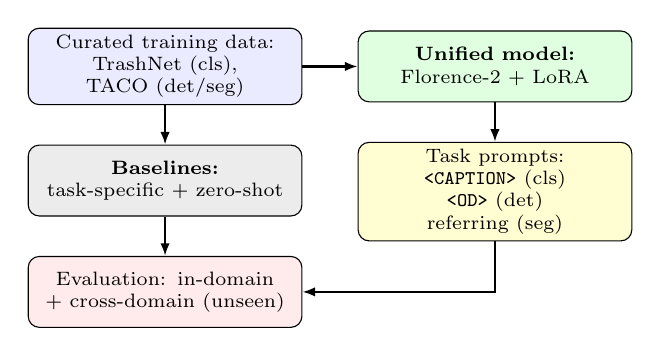
\begin{tikzpicture}[
  font=\scriptsize,
  node distance=5mm and 7mm,
  box/.style={draw, rounded corners, align=center, minimum height=9mm,
              text width=33mm, inner sep=2.5pt},
  arr/.style={-{Latex[length=1.6mm]}, thick},
]
\node[box, fill=blue!8] (data) {Curated training data:\\ TrashNet (cls), TACO (det/seg)};
\node[box, fill=green!12, right=of data] (flor) {\textbf{Unified model:}\\ Florence-2 + LoRA};
\node[box, fill=gray!15, below=of data] (s1) {\textbf{Baselines:}\\ task-specific + zero-shot};
\node[box, fill=yellow!18, below=of flor] (tasks) {Task prompts:\\ \texttt{<CAPTION>} (cls)\\ \texttt{<OD>} (det)\\ referring (seg)};
\node[box, fill=red!8, below=of s1] (eval) {Evaluation: in-domain\\ + cross-domain (unseen)};
\draw[arr] (data) -- (flor);
\draw[arr] (data) -- (s1);
\draw[arr] (s1) -- (eval);
\draw[arr] (flor) -- (tasks);
\draw[arr] (tasks.south) |- (eval.east);
\end{tikzpicture}
\caption{Study overview. Task-specific and zero-shot foundation models serve as
baselines. A single Florence-2 model is adapted with LoRA to perform all three
tasks via task prompts. All models are evaluated on both in-domain and
cross-domain data; cross-domain test sets are never seen during training.}
\label{fig:pipeline}
\end{figure}


\section{Methodology}
Fig.~\ref{fig:pipeline} summarizes our approach: a single vision-language foundation
model, adapted using low-rank parameters, that performs waste classification, object
detection, and segmentation through task-specific prompts. Notation is summarized in
Appendix~\ref{app:notation}.

\subsection{Problem Formulation}
We consider three waste-analysis tasks,
$\mathcal{T}=\{\textsc{cls},\textsc{det},\textsc{seg}\}$,
corresponding to material classification, object detection, and region segmentation.
Let $\mathcal{D}_{\text{in}}=\{(x_i,t_i,y_i)\}$ denote the training data, where
$x$ is an image, $t\in\mathcal{T}$ is a task identifier, and $y$ is the target:
a material label for \textsc{cls}, a set of labelled bounding boxes for \textsc{det},
or a set of annotated regions for \textsc{seg}. A separate dataset
$\mathcal{D}_{\text{out}}$ contains images from previously unseen waste environments
and is used exclusively for evaluation. Conventional approaches learn an independent
model $f_t$ for each task $t$. Instead, we seek a single model $f_\theta$ that
performs all tasks by conditioning on a task prompt $p_t$:
\begin{equation}
\hat{y} = f_\theta(x,\,p_t), \qquad t\in\mathcal{T}.
\label{eq:unified}
\end{equation}
The model is trained only on $\mathcal{D}_{\text{in}}$ and evaluated on both
in-domain and cross-domain data to measure generalization under domain shift.

\subsection{Unified Model: Florence-2}
We instantiate $f_\theta$ using Florence-2~\cite{florence2}, a vision-language
foundation model that formulates diverse vision tasks as a unified
sequence-generation problem. An image encoder converts the input $x$ into visual
tokens $v=\mathrm{Enc}_{\text{img}}(x)$, while the task prompt $p_t$ is represented
as text tokens. A shared encoder fuses the two representations, and an autoregressive
decoder generates the output sequence $\hat{y}=(\hat{y}_1,\ldots,\hat{y}_m)$ one
token at a time. Task behavior is determined entirely by the prompt: for
\textsc{cls}, Florence-2 generates a class label; for \textsc{det} and \textsc{seg},
it generates class names together with discretized location tokens
$\langle\text{loc}_i\rangle$ that encode spatial coordinates into $1000$ bins per
axis. Because all tasks share the same sequence-generation framework, a single
network can perform all three tasks while reusing common visual representations.

\subsection{Multi-Task Adaptation with LoRA}
Fine-tuning all parameters of Florence-2 is expensive and may reduce the generality
of the pre-trained model. We therefore use Low-Rank Adaptation
(LoRA)~\cite{lora}. For a frozen weight $W\in\mathbb{R}^{d\times k}$, LoRA learns
a low-rank update $\Delta W=BA$ with $B\in\mathbb{R}^{d\times r}$,
$A\in\mathbb{R}^{r\times k}$, and $r\ll\min(d,k)$, giving
\begin{equation}
W' = W + \tfrac{\alpha}{r}\,BA .
\label{eq:lora}
\end{equation}
Only $A$ and $B$ are optimized; the backbone remains frozen. Adapters are inserted
into $W_q,W_k,W_v,W_o$ of every attention layer in both the encoder and decoder,
with $r{=}16$ and $\alpha{=}32$. This trains only a few million parameters, a
$14$\,MB add-on on top of the frozen model. Appendix~\ref{app:lora} lists the
complete adapter configuration.

\subsection{Training Objective}
We construct a unified training set by combining examples from all tasks in
$\mathcal{D}_{\text{in}}$. Each example is paired with a task-specific prompt and
a tokenized target:
\begin{itemize}
\item \texttt{<CAPTION>} $\to$ material label,
\item \texttt{<OD>} $\to$ class names and bounding-box location tokens,
\item segmentation prompt $\to$ region polygons as location tokens.
\end{itemize}
The adapter parameters $\phi=\{A,B\}$ are optimized with the sequence
cross-entropy loss
\begin{equation}
\mathcal{L}(\phi) = -\!\!\sum_{(x,p_t,y)\in\mathcal{D}_{\text{in}}}\sum_{j=1}^{|y|}
\log P_\theta\!\left(y_j \mid y_{<j}, x, p_t\right),
\label{eq:loss}
\end{equation}
with the backbone frozen. Because all three tasks contribute gradients through the
same adapter parameters, the learned representations reflect all tasks rather than
any single objective.

\subsection{Inference}
At inference time the task prompt determines the output. For detection we use the
region-proposal head, which provides higher recall on cluttered waste scenes than
the standard \texttt{<OD>} head. For segmentation we use a two-stage procedure:
phrase grounding first identifies each waste instance, a segmentation head then
generates its mask, and all instance masks are merged into a single foreground map
for evaluation.

\section{Experimental Setup}
\textbf{Datasets.} Publicly available datasets are used for in-domain and
cross-domain evaluation. In-domain data are used for training; cross-domain data
are used exclusively for testing. Training uses TrashNet (classification) and TACO (detection and
segmentation). Cross-domain test sets are RealWaste and WaRP-C (classification),
Trash-ICRA19, ZeroWaste-f, and WaRP-D (detection), and DWSD and ZeroWaste-f
(segmentation). Tables mark these as \emph{(in)} and \emph{(cross)}.

\textbf{Baselines.} Task-specific (TS) models are trained on in-domain data for a
single task: ViT-Base, ResNet-50, EfficientNet-B0 (classification); YOLOv8m and
Faster R-CNN (detection); DeepLabV3+, U-Net, and Mask R-CNN (segmentation).
Foundation-model (FM) baselines are evaluated zero-shot: CLIP (classification),
Grounding DINO (detection), SAM (segmentation). Our unified model (UNI) is
Florence-2 with a shared LoRA adapter trained jointly across all tasks. Since UNI
is fine-tuned while FM baselines are zero-shot, we include a single-task ablation
(Section~\ref{sec:analysis}) to isolate the effect of joint training.

\textbf{Metrics.} Models share their task's metrics: accuracy and macro-F1
(classification), class-agnostic F1 at IoU\,0.5 (detection), and binary mIoU
(segmentation). Cross-domain labels are mapped to a shared TrashNet space
(Appendix~\ref{app:mapping}).

\textbf{Implementation.} The Florence-2 backbone is frozen; only LoRA parameters
are optimized with AdamW (learning rate $10^{-4}$, batch size~1, 3~epochs) on a
single NVIDIA A100 (40\,GB). Appendix~\ref{app:exp} details the full training and
evaluation.

\section{Results}

\subsection{Classification}

\begin{table}[htbp]
\caption{Classification: Accuracy \% (macro-F1)}
\label{tab:cls}
\begin{center}
\setlength{\tabcolsep}{3.5pt}
\footnotesize
\begin{tabular}{@{}llccc@{}}
\toprule
\textbf{Model} & \textbf{Reg.} & \textbf{TrashNet} & \textbf{RealWaste} & \textbf{WaRP-C} \\
 & & \textit{(in)} & \textit{(cross)} & \textit{(cross)} \\
\midrule
ViT-Base & TS & \textbf{96.44 (.957)} & 50.29 (.455) & 21.99 (.215) \\
EfficientNet-B0 & TS & 89.53 (.876) & 44.35 (.399) & 46.29 (.346) \\
ResNet-50 & TS & 80.83 (.771) & 23.42 (.183) & 17.28 (.164) \\
CLIP ViT-B/16 & FM & 67.83 (.586) & 58.02 (.521) & 43.07 (.395) \\
\textbf{Florence-2 FT} & UNI & 85.24 (.701) & \textbf{58.29 (.569)} & \textbf{60.35 (.415)} \\
\bottomrule
\end{tabular}
\end{center}
\footnotesize Each cell: accuracy \% (macro-F1). TS: task-specific; FM: foundation (zero-shot); UNI: unified.
\end{table}

As Table~\ref{tab:cls} shows, ViT-Base has the highest in-domain accuracy (96.44\%)
but falls to 50.29\% on RealWaste and 21.99\% on WaRP-C. On WaRP-C the unified Florence-2 is clearly best
(60.35\%), far ahead of the best task-specific model and of CLIP. On RealWaste it is highest
too (58.29\%), but here CLIP is very close (58.02\%); the unified model's lead is
clearer on macro-F1 (0.569 vs CLIP's 0.521).

\subsection{Detection}

\begin{table}[htbp]
\caption{Detection: F1 at IoU 0.5 (class-agnostic)}
\label{tab:det}
\begin{center}
\begin{tabular}{@{}llcccc@{}}
\toprule
\textbf{Model} & \textbf{Reg.} & \textbf{TACO} & \textbf{ICRA19} & \textbf{ZeroW.} & \textbf{WaRP-D} \\
 & & \textit{(in)} & \textit{(cross)} & \textit{(cross)} & \textit{(cross)} \\
\midrule
YOLOv8m & TS & \textbf{0.641} & 0.292 & 0.220 & 0.184 \\
Faster R-CNN & TS & 0.195 & 0.182 & 0.146 & 0.123 \\
Grounding DINO & FM & 0.253 & 0.268 & 0.208 & 0.192 \\
\textbf{Florence-2 FT} & UNI & 0.366 & \textbf{0.397} & \textbf{0.272} & \textbf{0.281} \\
\bottomrule
\end{tabular}
\end{center}
\end{table}

As Table~\ref{tab:det} reports, YOLOv8m is best in-domain (0.641 F1) but falls to
0.18--0.29 on unseen data, a drop of about 54--71\%. All methods struggle most on
underwater debris (Trash-ICRA19), where the task-specific model YOLOv8m (0.292)
and
the zero-shot Grounding DINO (0.268) end up close, and neither is strong. The unified
model is best on all three unseen detection sets (0.397, 0.272, 0.281), clearly ahead
of both baselines on each, joining foundation-model robustness with task-adapted
accuracy.

\subsection{Segmentation}
\vspace{-3mm}
\begin{table}[htbp]
\caption{Segmentation: Binary mIoU}
\label{tab:seg}
\begin{center}
\begin{tabular}{@{}llccc@{}}
\toprule
\textbf{Model} & \textbf{Regime} & \textbf{TACO} & \textbf{DWSD} & \textbf{ZeroWaste-f} \\
 & & \textit{(in)} & \textit{(cross)} & \textit{(cross)} \\
\midrule
DeepLabV3+ & TS & \textbf{0.454} & 0.152 & 0.132 \\
U-Net & TS & 0.329 & 0.126 & 0.131 \\
Mask R-CNN & TS & 0.289 & 0.156 & 0.169 \\
SAM ViT-H & FM & 0.038 & 0.149 & 0.027 \\
\textbf{Florence-2 FT} & UNI & 0.222 & \textbf{0.180} & 0.160$^{\mathrm{a}}$ \\
\bottomrule
\end{tabular}
\end{center}
\footnotesize $^{\mathrm{a}}$Statistical tie: paired Wilcoxon $p{=}0.98$; bootstrap 95\% CI of per-image difference includes 0 ($n{=}929$).
\end{table}

As Table~\ref{tab:seg} shows, segmentation has the smallest gaps. The task-specific
models also drop on unseen data
(DeepLabV3+ from 0.454 in-domain to 0.13--0.15), but they do not fall to near zero
like the classifiers and detectors do. The unified model is highest on DWSD (0.180
vs the best task-specific model's 0.156). On ZeroWaste-f it is tied with the best
task-specific model, Mask R-CNN (0.160 vs 0.169; paired Wilcoxon $p{=}0.98$, and the
bootstrap 95\% CI of the per-image difference includes zero). So on segmentation
the unified model still leads, but only by a small margin.

\begin{figure}[t]
\centering
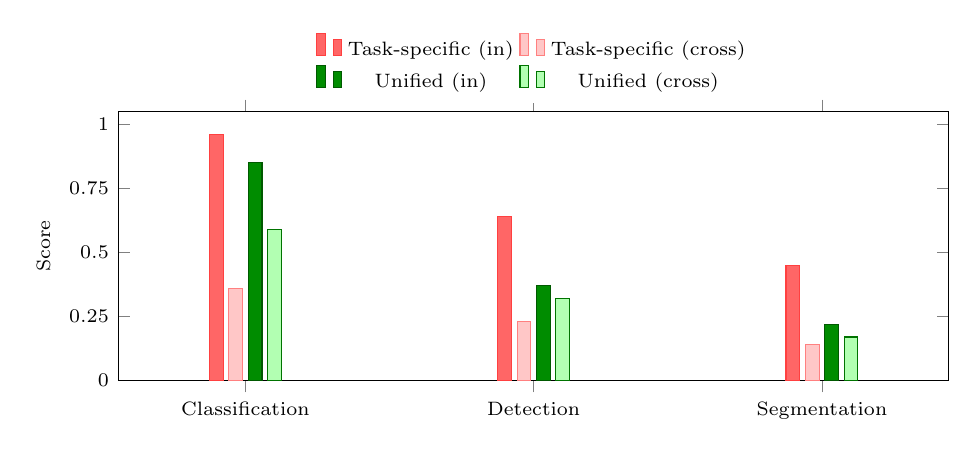
\begin{tikzpicture}
\begin{axis}[
    width=\columnwidth, height=5.0cm,
    ybar, bar width=5pt,
    enlarge x limits=0.22,
    ymin=0, ymax=1.05,
    ylabel={Score}, ylabel near ticks,
    symbolic x coords={Classification, Detection, Segmentation},
    xtick=data, x tick label style={font=\scriptsize},
    ytick={0,0.25,0.5,0.75,1.0},
    legend style={at={(0.5,1.03)}, anchor=south, legend columns=2,
                  font=\scriptsize, draw=none},
    tick label style={font=\scriptsize}, label style={font=\scriptsize},
]
\addplot+[ybar, fill=red!60, draw=red!75] coordinates
  {(Classification,0.96) (Detection,0.64) (Segmentation,0.45)};
\addplot+[ybar, fill=red!22, draw=red!50] coordinates
  {(Classification,0.36) (Detection,0.23) (Segmentation,0.14)};
\addplot+[ybar, fill=green!55!black, draw=green!35!black] coordinates
  {(Classification,0.85) (Detection,0.37) (Segmentation,0.22)};
\addplot+[ybar, fill=green!30, draw=green!45!black] coordinates
  {(Classification,0.59) (Detection,0.32) (Segmentation,0.17)};
\legend{Task-specific (in), Task-specific (cross), Unified (in), Unified (cross)}
\end{axis}
\end{tikzpicture}
\caption{In-domain vs cross-domain performance on all three tasks. Metrics:
accuracy (classification), F1 at IoU\,0.5 (detection), binary mIoU
(segmentation). Bar heights are comparable only within tasks.}
\label{fig:robust}
\end{figure}

\subsection{Summary}
On every unseen test set the unified Florence-2 is best or tied for best. The
margin is large where task-specific models collapse out of domain (classification,
detection) and small on segmentation and the hardest cross-domain sets, where a
strong rival stays close. Qualitative examples are shown in Appendix~\ref{app:qual}.

\section{Analysis and Discussion}
\label{sec:analysis}

\textbf{Is the gain from fine-tuning or from joining the tasks?}
We compare the unified model with Florence-2 adapters trained separately for each
task under the same evaluation protocol (Table~\ref{tab:ablation}). The unified
model achieves substantially better performance on classification and segmentation
and remains competitive on detection. Since the single-task adapters are also fine-tuned, gains
cannot be from fine-tuning alone. Jointly learning all three tasks enables the
model to exploit complementary information: material-recognition features also
support localization and boundary delineation.
\vspace{-3mm}
\begin{table}[htbp]
\caption{Single-task vs. unified Florence-2 (cross-domain), same protocol}
\label{tab:ablation}
\begin{center}
\begin{tabular}{@{}llcc@{}}
\toprule
\textbf{Task (benchmark)} & \textbf{Metric} & \textbf{Single-task} & \textbf{Unified} \\
\midrule
Classification (WaRP-C) & Acc \% & 39.97 & \textbf{60.35} \\
Segmentation (ZeroWaste-f) & mIoU & 0.130 & \textbf{0.160} \\
Segmentation (DWSD) & mIoU & 0.119 & \textbf{0.180} \\
Detection (ZeroWaste-f) & F1 & 0.257 & \textbf{0.272} \\
Detection (WaRP-D) & F1 & \textbf{0.300} & 0.281 \\
\bottomrule
\end{tabular}
\end{center}
\end{table}

\textbf{Accuracy vs. generalization.}
Task-specific models achieve the highest in-domain scores but experience substantial
performance degradation on unseen environments. In contrast, the unified model
sacrifices some in-domain accuracy while maintaining much stronger cross-domain
performance. As shown in Fig.~\ref{fig:robust}, the performance gap is consistently smaller
for the unified model. Using \emph{retention} (cross-domain / in-domain score),
task-specific models retain 31--37\% while the unified model retains 70--87\%,
showing that robustness comes from learning transferable representations rather
than maximizing in-domain accuracy.

\textbf{One model instead of many.}
The practical benefit of the proposed approach is deployment simplicity. The unified
model replaces a three-model pipeline (approximately 552~MB of weights) with a single
Florence-2 backbone and a lightweight 14~MB LoRA adapter. Task selection is performed
through prompts rather than model switching, reducing deployment and maintenance
overhead. The trade-off is inference speed: autoregressive decoding is slower than
specialized task-specific models. Consequently, the primary advantage of the unified
approach is simplified deployment and maintenance rather than maximum throughput.

\textbf{Understanding the generalization gains.}
Task-specific models optimize for a single dataset and task, degrading when
environments change (lighting, clutter, backgrounds, scale). Foundation models are
more robust through diverse pre-training but underperform in-domain. The unified
model combines both: LoRA specializes Florence-2 for waste while preserving its
broad visual knowledge. Although the exact mechanism requires further investigation,
jointly adapting across multiple tasks appears to encourage representations that
transfer more effectively under domain shift.

\section{Limitations}
Our work has two primary limitations. First, segmentation remains the weakest component of the framework because Florence-2 represents masks as coordinate sequences rather than dense pixel masks, which can reduce boundary precision in crowded scenes. As a result, its advantage over specialized segmentation models is relatively small. Second, the evaluation covers a limited set of waste datasets, and broader validation would strengthen the generality of the findings. All reported results are based on a single training run.
% , and evaluation across multiple random seeds would provide a more reliable estimate of performance variability.
These limitations are directions for future research.

\section{Conclusion}
We present a unified vision-language framework for automated waste management that performs classification, detection, and segmentation within a single prompt-driven architecture. By adapting Florence-2 with a lightweight LoRA module, the proposed model replaces multiple task-specific pipelines with a single deployable system. Across seven real-world waste datasets, the unified model consistently matches or outperforms task-specific and zero-shot foundation-model baselines, particularly under cross-domain evaluation. Our ablation study further shows that these gains arise primarily from joint multi-task adaptation rather than fine-tuning alone. Overall, the results suggest that lightly adapted vision-language foundation models provide a practical and robust solution for waste analysis in diverse real-world environments. Future work will explore broader waste-analysis tasks, larger and more diverse datasets, and improved segmentation strategies.

\phantomsection
\label{sec:ack}
\section*{Acknowledgments}
The assistance of Claude (Anthropic)~\cite{claude} was used for rephrasing the content and general \LaTeX\ formatting. The introduction and all other sections,
including the core methodology, experimental configurations, results, and
conclusions, were developed solely by us. We remain fully accountable
for the final content.

\begin{thebibliography}{00}
\bibitem{florence2} B. Xiao, H. Wu, W. Xu, et al., ``Florence-2: Advancing a unified representation for a variety of vision tasks,'' in \textit{Proc. CVPR}, 2024.
\bibitem{lora} E. J. Hu, Y. Shen, P. Wallis, et al., ``LoRA: Low-rank adaptation of large language models,'' in \textit{Proc. ICLR}, 2022.
\bibitem{peft} S. Mangrulkar, S. Gugger, L. Debut, et al., ``PEFT: State-of-the-art parameter-efficient fine-tuning methods,'' Hugging Face, 2022.
\bibitem{taco} P. F. Proen\c{c}a and P. Sim\~oes, ``TACO: Trash annotations in context for litter detection,'' arXiv:2003.06975, 2020.
\bibitem{trashnet} M. Yang and G. Thung, ``Classification of trash for recyclability status,'' Stanford CS229 Project, 2016.
\bibitem{realwaste} S. Single, S. Iranmanesh, and R. Raval, ``RealWaste: A novel real-life data set for landfill waste classification using deep learning,'' \textit{Information}, 2023.
\bibitem{icra19} M. Fulton, J. Hong, M. J. Islam, and J. Sattar, ``Robotic detection of marine litter using deep visual detection models,'' in \textit{Proc. ICRA}, 2019.
\bibitem{zerowaste} D. Bashkirova, M. Abdelfattah, Z. Zhu, et al., ``ZeroWaste dataset: Towards deformable object segmentation in cluttered scenes,'' in \textit{Proc. CVPR}, 2022.
\bibitem{warp} D. Yudkin, et al., ``WaRP: Waste recycling plant dataset for detection, classification, and segmentation,'' 2022.
\bibitem{dwsd} A. Ali, S. Acharjee, M. M. Sk., S. Z. Alharthi, S. Sinha Chaudhuri, and A. Akhunzada, ``DWSD: Dense waste segmentation dataset,'' \textit{Data in Brief}, vol. 59, art. 111340, 2025.
\bibitem{clip} A. Radford, J. W. Kim, C. Hallacy, et al., ``Learning transferable visual models from natural language supervision,'' in \textit{Proc. ICML}, 2021.
\bibitem{gdino} S. Liu, Z. Zeng, T. Ren, et al., ``Grounding DINO: Marrying DINO with grounded pre-training for open-set object detection,'' in \textit{Proc. ECCV}, 2024.
\bibitem{sam} A. Kirillov, E. Mintun, N. Ravi, et al., ``Segment anything,'' in \textit{Proc. ICCV}, 2023.
\bibitem{vit} A. Dosovitskiy, L. Beyer, A. Kolesnikov, et al., ``An image is worth 16x16 words: Transformers for image recognition at scale,'' in \textit{Proc. ICLR}, 2021.
\bibitem{resnet} K. He, X. Zhang, S. Ren, and J. Sun, ``Deep residual learning for image recognition,'' in \textit{Proc. CVPR}, 2016.
\bibitem{efficientnet} M. Tan and Q. Le, ``EfficientNet: Rethinking model scaling for convolutional neural networks,'' in \textit{Proc. ICML}, 2019.
\bibitem{yolov8} G. Jocher, A. Chaurasia, and J. Qiu, ``Ultralytics YOLOv8,'' 2023.
\bibitem{fasterrcnn} S. Ren, K. He, R. Girshick, and J. Sun, ``Faster R-CNN: Towards real-time object detection with region proposal networks,'' in \textit{Proc. NeurIPS}, 2015.
\bibitem{unet} O. Ronneberger, P. Fischer, and T. Brox, ``U-Net: Convolutional networks for biomedical image segmentation,'' in \textit{Proc. MICCAI}, 2015.
\bibitem{deeplab} L.-C. Chen, Y. Zhu, G. Papandreou, F. Schroff, and H. Adam, ``Encoder-decoder with atrous separable convolution for semantic image segmentation,'' in \textit{Proc. ECCV}, 2018.
\bibitem{maskrcnn} K. He, G. Gkioxari, P. Doll\'ar, and R. Girshick, ``Mask R-CNN,'' in \textit{Proc. ICCV}, 2017.
\bibitem{babe} A. Bab\'e, R. Cuingnet, M. Scuturici, and S. Miguet, ``Generalization abilities of foundation models in waste classification,'' 2023.
\bibitem{claude} Anthropic, ``Claude,'' large language model, 2025. [Online]. Available: https://www.anthropic.com/claude
\end{thebibliography}



\appendices

\section{Notation}
\label{app:notation}
Table~\ref{tab:notation} summarizes the symbols used in
Eqs.~\eqref{eq:unified}--\eqref{eq:loss} and throughout the methodology.

\begin{table}[htbp]
\caption{Summary of notation}
\label{tab:notation}
\begin{center}
\setlength{\tabcolsep}{4pt}
\footnotesize
\begin{tabular}{@{}ll@{}}
\toprule
\textbf{Symbol} & \textbf{Meaning} \\
\midrule
$\mathcal{T}$ & Task set $\{\textsc{cls},\textsc{det},\textsc{seg}\}$ \\
$t$ & Task identifier, $t\in\mathcal{T}$ \\
$x$ & Input image \\
$p_t$ & Text prompt selecting task $t$ \\
$y$ & Ground-truth target (label / boxes / regions) \\
$\hat{y}$ & Model output sequence $(\hat{y}_1,\ldots,\hat{y}_m)$ \\
$f_\theta$ & Unified model with parameters $\theta$ \\
$\mathcal{D}_{\text{in}}$ & In-domain training data $\{(x_i,t_i,y_i)\}$ \\
$\mathcal{D}_{\text{out}}$ & Cross-domain (unseen) evaluation data \\
$v$ & Visual tokens, $v=\mathrm{Enc}_{\text{img}}(x)$ \\
$\langle\text{loc}_i\rangle$ & Discretized location token (1000 bins/axis) \\
\midrule
$W$ & Frozen pre-trained weight, $W\in\mathbb{R}^{d\times k}$ \\
$W'$ & LoRA-adapted weight \\
$\Delta W{=}BA$ & Low-rank update \\
$B,A$ & LoRA factors, $B\in\mathbb{R}^{d\times r}$, $A\in\mathbb{R}^{r\times k}$ \\
$r$ & LoRA rank ($r{=}16$), $r\ll\min(d,k)$ \\
$\alpha$ & LoRA scaling factor ($\alpha{=}32$) \\
$d,k$ & Output / input dimensions of $W$ \\
$\phi{=}\{A,B\}$ & Trainable adapter parameters \\
$\mathcal{L}(\phi)$ & Sequence cross-entropy training loss \\
$P_\theta(\cdot)$ & Token probability under the model \\
$|y|$ & Target sequence length \\
\bottomrule
\end{tabular}
\end{center}
\end{table}

\section{LoRA Configuration}
\label{app:lora}
We adapt Florence-2-large-ft~\cite{florence2} with LoRA~\cite{lora} using the
PEFT library~\cite{peft}. Low-rank adapters are inserted into the query, key,
value, and output projections ($W_q,W_k,W_v,W_o$) of every multi-head attention
layer in both the encoder and the decoder. We use rank $r{=}16$, scaling
$\alpha{=}32$ (so the effective update is scaled by $\alpha/r{=}2$), and dropout
$0.05$. The backbone weights remain frozen; only the LoRA factors $A$ and $B$ are
trained, which corresponds to a few million parameters and a $14$\,MB adapter on
top of the frozen $0.77$\,B-parameter model. $B$ is initialized to zero and $A$ to
a random Gaussian, so the adapted model is identical to the pre-trained model at
the start of training.

\section{Experimental Procedure}
\label{app:exp}
\textbf{Unified training data.} We merge the three task datasets into a single
prompt--target corpus. Each \textsc{cls} example uses the \texttt{<CAPTION>}
prompt with the material label as target; each \textsc{det} example uses the
\texttt{<OD>} prompt with class names and bounding-box location tokens; each
\textsc{seg} example uses a referring-segmentation prompt with region polygons
encoded as location tokens. Examples from all tasks are shuffled together so that
every mini-batch may contain different tasks.

\textbf{Optimization.} The LoRA parameters are optimized with AdamW (learning
rate $10^{-4}$, weight decay default) for $3$ epochs, with per-device batch
size~$1$ and gradient accumulation of $8$ (effective batch size~$8$). Training
uses a single NVIDIA A100 (40\,GB). The same configuration is used for the
single-task ablation adapters, which differ only in their training data.

\textbf{Inference.} For detection we decode with the class-agnostic
region-proposal head, which gives higher recall on cluttered waste scenes than
the standard \texttt{<OD>} head. For segmentation we use a two-stage cascade:
phrase grounding locates each waste instance, the segmentation head produces its
mask, and the instance masks are merged into a single binary foreground map for
mIoU. As a concrete example, a detection output decodes as a token sequence such
as \texttt{bottle <loc\_512><loc\_640><loc\_734><loc\_898>}, where the four
location tokens are the quantized box corners; segmentation replaces the box with
a longer polygon of location tokens.

\textbf{Evaluation protocol.} In-domain test splits come from the training
datasets (TrashNet, TACO); cross-domain test sets are never seen during training.
For cross-domain classification, dataset-specific labels are mapped into the
shared TrashNet material space before scoring. Detection uses class-agnostic F1 at
IoU$\,{\geq}\,0.5$; segmentation uses binary (foreground/background) mIoU. For the
ZeroWaste-f segmentation comparison we additionally report a paired Wilcoxon
signed-rank test and a bootstrap $95\%$ confidence interval over per-image score
differences ($n{=}929$) to assess whether the gap to the strongest baseline is
significant.

\section{Qualitative Results}
\label{app:qual}
Fig.~\ref{fig:qual} shows cross-domain predictions of the unified model and the
strongest task-specific baseline on unseen images, with per-image scores.

\begin{figure*}[!t]
\centering
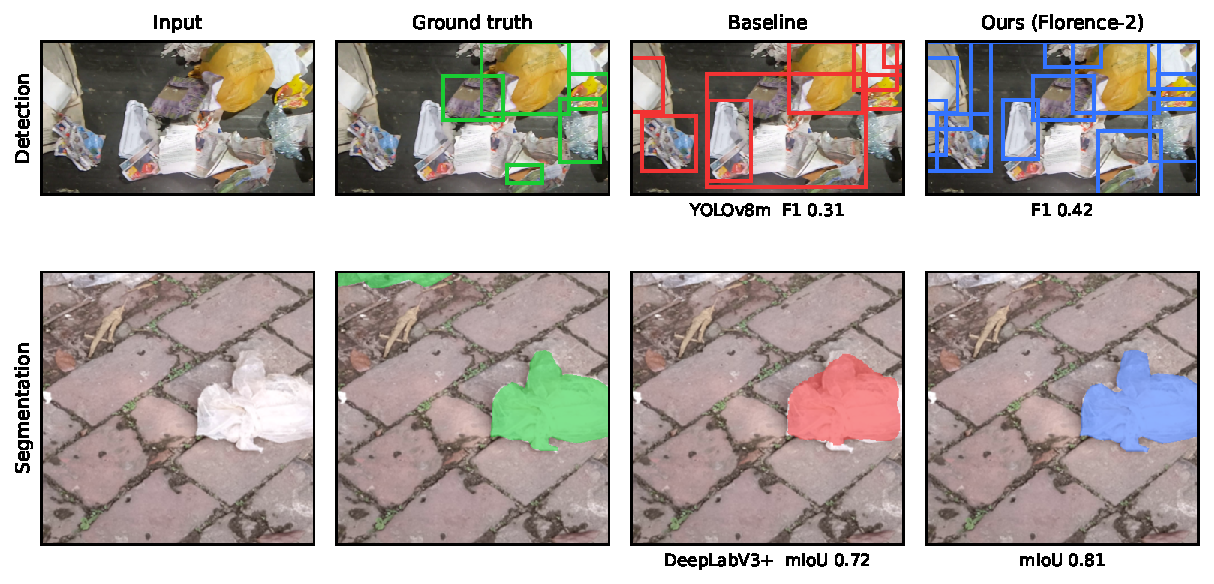
\includegraphics[width=\textwidth]{qualitative_panel.pdf}
\caption{Qualitative comparison on unseen mixed-waste imagery.
\emph{Top---detection:} the unified model (Florence-2, blue) achieves higher
class-agnostic F1 than the YOLOv8m baseline (red), improving from 0.31 to 0.42.
\emph{Bottom---segmentation:} predicted masks are compared against the ground-truth
mask; the unified model yields a tighter object boundary, raising mIoU from 0.72 to
0.81. Columns: input, ground truth (green), baseline (red), ours (blue).}
\label{fig:qual}
\end{figure*}

\section{Cross-Domain Label Mapping}
\label{app:mapping}
Because each dataset uses its own label set, cross-domain classification scores
the predicted material against a shared TrashNet category space. \textbf{RealWaste}
(9 classes) maps six classes one-to-one---\textsc{cardboard}, \textsc{glass},
\textsc{metal}, \textsc{paper}, \textsc{plastic}, and ``miscellaneous trash''
$\to$ \textsc{trash}; the remaining three (food organics, textile trash,
vegetation) have no TrashNet equivalent and are excluded, leaving $3{,}587$ test
images. \textbf{WaRP-C} is mapped as in Table~\ref{tab:warpc-map}, yielding
$1{,}551$ test images. No mapping is needed for detection or segmentation, which
are evaluated class-agnostically.

\begin{table}[htbp]
\caption{WaRP-C $\to$ TrashNet label mapping}
\label{tab:warpc-map}
\begin{center}
\footnotesize
\begin{tabular}{@{}ll@{}}
\toprule
\textbf{WaRP-C class} & \textbf{TrashNet category} \\
\midrule
bottle, detergent (bottles), canister & plastic \\
cans & metal \\
cardboard & cardboard \\
\bottomrule
\end{tabular}
\end{center}
\end{table}

\end{document}